\documentclass[language=en,12pt]{aghdpl}
% \documentclass[language=en,11pt]{aghdpl}  % praca w języku angielskim
\usepackage{listings}
\usepackage{hyperref}
\usepackage{listings-rust}
%---------------------------------------------------------------------------

\author{Mateusz Domalewski}
\shortauthor{M. Domalewski}

%\titlePL{Przygotowanie bardzo długiej i pasjonującej pracy dyplomowej w~systemie~\LaTeX}
%\titleEN{Preparation of a very long and fascinating bachelor or master thesis in \LaTeX}

\titlePL{Poszukiwanie sygnatur kodu w zmapowanej pamięci procesu}
\titleEN{Analysis of code signatures in mapped memory of a process}


\shorttitlePL{Poszukiwanie sygnatur kodu w zmapowanej pamięci procesu} % skrócona wersja tytułu jeśli jest bardzo długi
\shorttitleEN{Analysis of code signatures in mapped memory of a process}


% Dopuszczalne wartości[1,2]:
% * "Projekt dyplomowy" - na koniec studiów I stopnia
% * "Praca dyplomowa" - na koniec studiów II stopnia
% [1] Zasady dyplomowania w roku akademickim 2020/2021 (Decyzja Dziekana WEAIiIB nr 16/2020 z dnia 9 grudnia 2020 roku)
% [2] Załącznik nr 1a) do Decyzji nr 16/2020 Dziekana Wydziału EAIiIB z dnia 09 grudnia 2020 r.
\thesistype{Engineering Thesis}
%\thesistype{Master of Science Thesis}

\supervisor{dr hab. inż. Krzysztof Rzecki}
%\supervisor{Paweł Kłeczek, PhD}

\degreeprogramme{Computer Science}
%\degreeprogramme{Automatics and Robotics}

\date{2024}

%\department{Katedra Informatyki Stosowanej}
%\department{Department of Applied Computer Science}

%\faculty{Wydział Elektrotechniki, Automatyki, Informatyki i Inżynierii Biomedycznej}
\faculty{Faculty of Electrical Engineering, Automatics, Computer Science and Biomedical Engineering}

\acknowledgements{"Everything is open source when you can read assembly"}


\begin{document}

	\titlepages
	\RedefinePlainStyle
	
	\setcounter{tocdepth}{2}
	\begin{abstract}

    As cybersecurity attacks are getting more and more complicated and avoid detection by hiding closer and closer to the operating system, memory analysis of a running process is a logical next step in research and protection against such threats.
    The research goal of this project is to research information about the Linux systems file based process interface, and find possible methods of extracting and parsing said information.
    The research is then applied in creation of a program performing analysis and allowing for manual introspection into the memory of a running process.
    As the tool and the paper showcases even the fundamental analysis of the running process internals can provide deep and meaningful insights about the system of origin, dependencies, architecture or even optimalizations and microcode used.
    This tool and research can be later used and extended to deepen and extend active threat protection and analysis at almost the kernel level.

\end{abstract}
	\tableofcontents
	\clearpage
    
	\chapter{Introduction}
\label{cha:intro}

\subsection{Background}

This study's purpose originates from a Cybersecurity background, and the need for monitoring of low level systems. 
Reverse engineering and binary analysis are prominent fields of cybersecurity and analyzing the code that is being run directly on the system level has recently gained much more traction. 
This can mostly due to recent ssh backdoor being uncovered \cite{collin_xz_2024} and it's possible high severity. 
Additionally this vulnerability was introduced at an extremely low level - by substituting an indirect function call by the operating system \cite{freund_oss-security_2024}. 
This highlights how a cleverly injected payload can bypass most of the lowest level security checks by making the program vulnerable by injecting malicious content at the linking stage.

The problem this thesis and project aims to provide the answer to is peering into the internal memory of a running process and ascertaining information about how does the actual mapped memory correspond to the parts that were used in process initialization.

\subsection{Significance}

As the \verb|/proc| filesystem provides a very powerful, but immensely low-level access to the processes of the linux system. \cite{kerrisk_proc_2010}
The produced tool that can be used to easily perform a task that would normally be obtained by a chain of command line methods (e.g. dump memory, decompile memory, decompile source, compare) makes the analysis and security assesment of a running process a much easier task. 
Additionally the exploration to determine which signatures can be determined from the running process memory should provide useful insights into what threats may be encountered at such low level and how can one protect against them.

%---------------------------------------------------------------------------

\section{Project Goals}
\label{sec:goals}

\subsection{Research Objectives and Questions}

This project's core objective are
\begin{enumerate}
    \item Gain information on how contents of a \verb|\proc| filesystem interface can be analyzed
    
    \item Create an abstraction over the aforementioned interface as well as the source files that were used to construct the contents of the process memory

    \item Create a tool which using the created abstraction can provide insight and analysis into the running process memory
    
    \item Ensure that the produced tool does not harm the running process and only is used to inspect its contents

\end{enumerate}

During the implementation of the tool and accompanying research the following questions should be answered:

\begin{enumerate}
    \item  how do modern operating systems protect themselves from memory-based attacks
    
    \item  how do the aforementioned memory protections influence the structure of the process memory
    
    \item  how does the modern linking process work and what dangers does it present
    
    \item  How are parts of program source and dependencies translate into the process memory, can this process be influenced and/or decrypted?
\end{enumerate}

%---------------------------------------------------------------------------

\section{Architecture}
\label{sec:architecture}

\subsection{Target}

The tool should target Linux-based systems which provide the \verb|/proc| filesystem interface. 
The primary architecture that the solution should target is x86\_64 based systems.
The tool should be usable as a standalone binary which should provide user with an readable interface that can be navigated.

\subsection{Architecture pattern}

As the app's functionality is dependent on multiple components that depend on each other but can be separated excluding some common communication the service architecture was chosen for the task.
As seen in the service diagram \ref{fig:modules} the tool should be comprised of three different modules.
The reader module will be the most basic one which will interact with the process and the linked libraries and parse their contents. The Analyzer module will call on the reader module to provide the desired output which it will use to provide insights about the data read. The last module will be responsible for the interaction with the user and should provide a way for the user to interact with the generated insights.

\begin{figure}
    \centering
    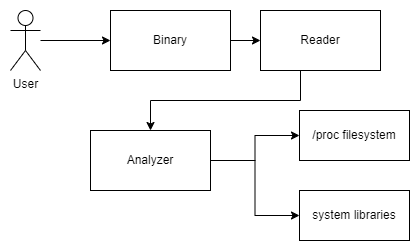
\includegraphics[width=0.5\linewidth]{modules.drawio.png}
    \caption{The user, modules, system and their interaction}
    \label{fig:modules}
\end{figure}

\subsection{Technologies used}

Due to the tool's low level access and safety requirements the Rust programming language seems as the obvious choice as it is a safe systems-level language which also provides a rich typesystem and cargo - rust's integrated build tool and dependency manager. 
Furthermore the language's vast ecosystem of open source packages (also known as crates) the project can make use of many useful tools to ease the development process.
Lastly rust's borrow checker rules \cite{TODO} enforce program's memory safety which is crucial with interacting within such volatile environments.

\subsection{Limitations}

\begin{enumerate}
    \item The \verb|\proc| filesystem is not part of the UNIX standard \cite{kerrisk_proc_2010} and therefore the tool can be used only on Linux systems which expose it
    \item Different architectures even from the same chip manufacturer can have different instruction sets \cite{intel_corporation_intel_2024}
    \item Sometimes the function and symbol definitions can be mangled or even deliberately erased which limits the tool's usability
    \item Decompilation reverse engineering and binary analysis is a broad subdiscipline of cybersecurity and with scope to broad to fully include in such project
\end{enumerate}

	\chapter{Literature Overview}
\label{cha:lit_overview}

\section{Theoretical Framework}

As the thesis is in nature a research and experimental project the theory will mostly be used as a reference in how internals of the Linux system work and how to approach analyzing them.

\section{Key Studies}

\begin{enumerate}
    \item{Linux manual pages}

    These pages can be accessed via any Linux distribution, but thanks to efforts by Michael Kerrisk they are also available online.
    These pieces of documentation are key in understanding specific Linux system concepts and how the system components work and interact with each other.

    \item Open source libraries and their documentation Due to the Rust and Linux system's open source licensing, most of the libraries in the ecosystem are not only open source but also very well documented.
    This proved extremely helpful, as it allowed for ease of use and swift integration of dependencies into the project.
    Additionally, with the code of the said libraries being open source peeking at the intrinsics of the Linux system code or the GNU dynamic linker \cite{noauthor_sourcewareorg_nodate} proved immensely helpful.

    \item The Linux Programming interface \cite{kerrisk_linux_2010}

    This book from Michael Kerrisk provides deep and example-backed information on almost every aspect of modern Linux systems.
    For the purpose of this project the secions on the \verb|\proc| filesystem as well as linux processes and their intrinsics proved crucial to understanding the backend from which the created tool reads and parses information

    \item How to write shared libraries \cite{drepper_how_2011}

    A great piece by the core author of the GNU dynamic linker which provides deep insights into the workings of the linux dynamic shared objects, their different properties and how authors of shared libraries should go about tailoring their code for better use.
    
\end{enumerate}

\section{Key Concepts}

\begin{enumerate}
    \item {Processes and how they're created}
Process at its core is a single instance of the program being executed.
    Before a program begins execution the operating system creates the process by allocating memory space, crating and addressing space within it, and loading all of the necessary program code and it's dependencies into the created memory.
    Furthermore in case of the systems that this project targets the process creation also involves loading separately and altering addresses of functions from the programs dependencies dynamically (dynamic linking).
    
    \item{The /proc filesystem}
    The modern Linux system exposes a special \verb|/proc| directory.
    This is an interface that allows for file-based access to process memory and information.
    As an example, in a system that is currently running a process with a designated id of 2240 the system will provide a \verb|\proc\2240| directory which will contain file interfaces for process memory, mappings, information and other invaluable pieces of information.
    However, this directory is ephemeral - meaning its contents can change and it will be destroyed upon the process' termination.

    \item{ Rust language concepts}
As the project is implemented in the rust programming language, knowledge of some basic language concepts will enhance further readability for people unfamiliar with the language (more in the rust book \cite{klabnik_rust_2023} or the language repo \cite{rust_foundation_rust-langrust_2024}): 

\subitem Struct - a data structure it can have public and private fields, does not inherently contain any functions but traits and other functionality can be implemented for it

    \subitem Enum - a type composed of multiple types. Rust's extensive enum types can contain types within their variant or implement traits.
    
    \subitem Trait - similar to an interface defines a shared functionality, however, with some caveats. For the purpose of this text, treating it as so should suffice.
    
    \subitem Macros - rust makes extensive use of macros for generating code (e.g. \verb|#[derive(debug)]| to automatically create a debug printable view of the struct) or providing extra functionality, for example, the \verb|matches!| macro to quickly verify whether the enum is of specific type 
\end{enumerate}
	\chapter{Solution Overview}
\label{cha:implementation}


\section{A note on modularity}

The project as a whole was designed to be an application that allows for code analysis, however, implementing abstractions from a level of reading bytes from process memory all the way to managing the interface's state resulted in the decision to split the deliverable into three separate entities named: reader, analyzer, and bin (for binary). As the project was implemented in rust, i was able to leverage rust's \verb|cargo| build system to easily manage all three projects as subdirectories

\begin{lstlisting}[caption="The basic project structure"]
/memspotter
    /reader
    /analyzer
    /bin
\end{lstlisting}

Furthermore, to ease the usage and possible refactors i decided to use rust's \verb|trait| \footnote{\enquote{Traits are similar to a feature often called interfaces in other languages, although with some differences.} - The Rust Book \cite{klabnik_traits_2023}} system to define shared function and type signatures which i could then implement for the data structures and abstractions of my choosing.

\begin{lstlisting}[caption=\label{lst:arch}"a trait definition example", language=Rust,]
/// Defines an architecture for the program
#[blanket::blanket(derive(Ref, Rc, Arc, Box))]
pub trait Arch: Debug + Clone + PartialEq + Eq {
    /// the process id type usually a [u64]
    type Pid: Sized + Debug;
    /// the single instruction type
    type Instruction: Sized + Debug + From<u8>;
    /// the header type of the /maps file for the arch
    type Header: MapHeader;
}    
\end{lstlisting}

as seen in \autoref{lst:arch} the Arch trait can even define no new functions but allow for defining that each architecture has an associated process id (or pid), instruction, and header types. This in turn can be used to ease the later abstractions. 

\begin{lstlisting}[caption=\label{lst:segment}"The memory segment trait", language=Rust]
/// generic trait for a allocated memory segment of a process
pub trait MemorySegment<A>: Sized + std::fmt::Debug + Clone + Eq + PartialEq
where
    A: Arch,
{
    /// returns the segment's bytes
    fn memory(&self) -> &[u8];
    /// iterates over the segment's bytes
    fn iter_memory(&self) -> impl Iterator<Item = &u8>;
    /// returns the segment's header
    fn header(&self) -> &A::Header;
}
\end{lstlisting}

A great example of such ease would be the memory segment trait \autoref{lst:segment} which can just take a given architecture implementation and it's specific header type will be included too, and can even be referenced in the function signatures (see the \verb|header(&self)| function).

Such design choice additionally allows for different implementations to expose a common interface but also be extremely flexible in the implementations, as, for example, the apple-based \verb|Mach-O| objects can implement it only for their own specific architecture, but the \verb|x86_64| family of systems can implement header for both the 64 and 32-bit ELF file variations. Furthermore, it also allows for easy differentiation between globally shared behavior and architecture-specific implementation, as can be seen in \autoref{lst:reader_structure}.

\begin{lstlisting}[caption=\label{lst:reader_structure}"Structure of the reader module outlining separate trait and implementation folder"]
/reader
    ...
    /traits
        arch.rs
        map.rs
        header.rs
        function.rs
        library.rs
        ...
    /x864_64
        arch.rs
        map.rs
        header.rs
        so_function.rs
        shared_object.rs
        ...
        
\end{lstlisting}

\section{Reader module}
\label{reader}

\subsection{Traits}

\begin{figure}
    \centering
    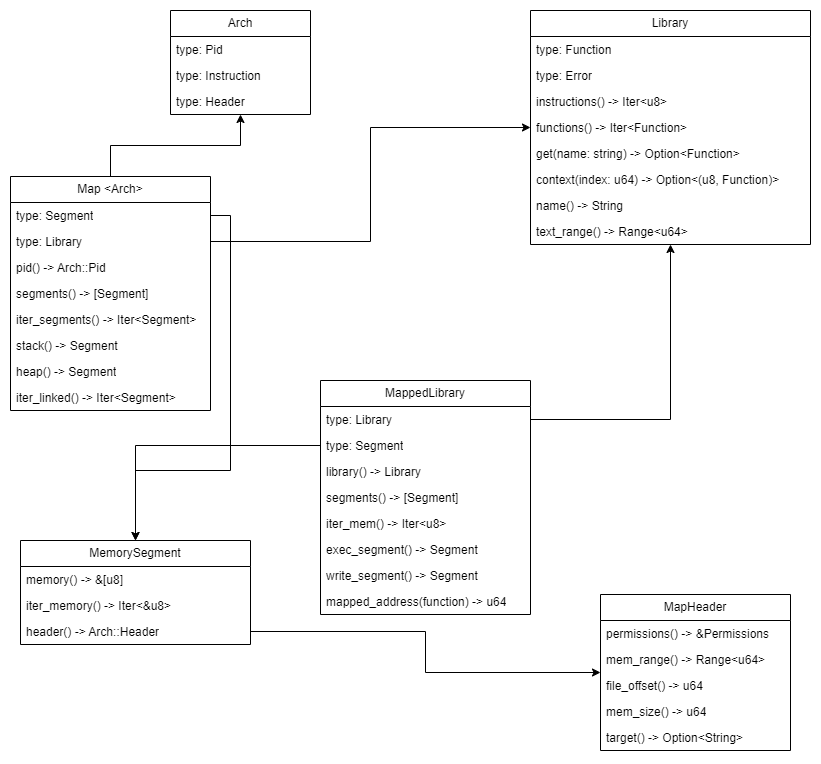
\includegraphics[width=0.65\linewidth]{reader_traits.drawio.png}
    \caption{Basic Diagram of Reader module trait dependencies and methods}
    \label{fig:reader-traits}
\end{figure}

The reader module at its core beside the Arch \autoref{lst:arch} and Segment \autoref{lst:segment} traits is represented by a total of 6 traits which dependence can be observed in \autoref{fig:reader-traits}.

    \subsubsection{Map}
    \label{reader:map}

The map is the most top-level trait and fully abstracts the contents of the entire process memory as well as the linked library code.
This trait allows access to the pid value of the process and the individual memory segments described and read from the \verb|\proc\{pid}\maps| \cite{kerrisk_proc_pid_maps5_2024} specification.
It also allows the user to access the individual mapped libraries of the process \autoref{reader:mapped_lib}.
It also defines special functions which return the special stack and heap segments \cite{kerrisk_memory_2010}.
    
\begin{lstlisting}[caption=\label{lst:map}"The Memory Map Trait definition", language=Rust]
 /// Describes a mapping of process part header to memory segments
#[blanket::blanket(derive(Ref, Rc, Arc, Box))]
pub trait Map<A: Arch + 'static>: Sized + Clone {
    /// map error type
    //type Error: std::error::Error;
    /// the specific memory segment type
    type Segment: MemorySegment<A>;
    /// the specific library type
    type Library: MappedLibrary<A>;

    /// returns the process pid
    fn pid(&self) -> A::Pid;

    /// returns segments
    fn segments(&self) -> Vec<Self::Segment>;
    /// returns an iterator ov the segments
    fn iter_segments(&self) -> impl Iterator<Item = Self::Segment>;

    /// returns the stack segment
    fn stack(&self) -> Self::Segment;
    /// returns the head segment
    fn heap(&self) -> Self::Segment;

    /// returns all segments that are linked
    //fn linked(&self) -> &[Self::Library];
    /// iterates over all segments that are linked
    fn iter_linked(&self) -> impl Iterator<Item = Self::Library>;
}   
\end{lstlisting}

 \subsubsection{MappedLibrary}
 \label{reader:mapped_lib} 

    This trait is an abstraction that represents a system-shared library that has been mapped onto segments of a running process.
    It defines methods that expose the actual library \autoref{reader:library} as well as the ability to access individual memory segments \autoref{lst:segment}.
    For ease of use in analysis it also defines methods for directly accessing the writeable and executable segments directly, as well a function which allows for translating the address of a library's function \autoref{reader:function} to an address in the process memory space.
\begin{lstlisting}[caption=\label{lst:mapped_lib}"The MappedLibrary Trait definition", language=Rust]
 /// represents a memory segment that is linked from some library
#[blanket::blanket(derive(Ref, Rc, Arc, Box))]
pub trait MappedLibrary<A>
where
    A: Arch,
    Self: std::fmt::Debug + Clone,
{
    /// the library type that the segment is mapped to
    type Library: Library<A>;
    /// the memory segment type to which the library refers
    type Segment: MemorySegment<A>;
    /// returns the linked library reference
    fn library(&self) -> Self::Library;
    /// returns all of the segments
    fn segments(&self) -> Vec<Self::Segment>;
    /// iterates over the whole linked memory
    /// goes through segments in order, so breaks between addressed 
    /// will not be included
    fn iter_mem(&self) -> impl Iterator<Item = &u8>;

    /// retrieves the first found executable segment
    /// CAN PANIC
    fn exec_segment(&self) -> Self::Segment;
    /// retrieves the first found writable segment
    /// CAN PANIC
    fn write_segment(&self) -> Self::Segment;
    /// returns the mapped address of a function
    fn mapped_address(&self, func: &<Self::Library as Library<A>>::Function) -> u64;
}   
\end{lstlisting}
  
    \subsubsection{Library}
     \label{reader:library} 
    
    This trait is a step lower on the abstraction ladder as it allows for the interaction with a shared library object.
    It exposes a definition of a specific implementation of the Function\autoref{reader:function} trait that the library uses as well as methods that allow dumping the entire executable section memory, as well as access to the range of the \verb|.text| section of the library file which holds the assembly code for the library's functions \cite{kerrisk_memory_2010}.
    Furthermore, this trait allows for getting the function code from the library object for a function with a specific name as well as some helper methods such as \verb|fn name(&self) -> String| which returns the name of the shared library for ease of use.
    
\begin{lstlisting}[caption=\label{lst:library}"The Library Trait definition", language=Rust]
/// Trait for interacting with binary linkable objects e.g. `.so` files
#[blanket::blanket(derive(Ref, Rc, Arc, Box))]
pub trait Library<A: Arch>: Debug + Sized + PartialEq + Eq + Clone {
    /// the type for an individual library function
    type Function: Function<A>;
    /// type for the error the trait can return in functions
    type Error: std::error::Error;
    /// returns an [Iterator] over all instructions
    /// most likely in instruction order but not guaranteed
    fn instructions(&self) -> impl Iterator<Item = A::Instruction>;
    /// returns all [Self::Function]s contained in the library
    fn functions(&self) -> impl Iterator<Item = Self::Function>;
    /// returns a [Self::Function] for a given name if exists
    /// else returns [None]
    fn get(&self, name: &str) -> Option<&Self::Function>;
    /// returns the instruction [u8] and the [Self::Function] for a given index if inside library
    /// bounds
    fn context(&self, index: u64) -> Option<(&A::Instruction, &Self::Function)>;

    /// returns the file name of the library
    fn name(&self) -> String;

    ///returns the file address range for the `.text` section
    fn text_range(&self) -> std::ops::Range<u64>;
}
\end{lstlisting}  

    \subsubsection{Function}
    \label{reader:function} 
    
    This trait defines the shared behavior of the functions that a given library contains.
    It allows for both direct assembly code access to the whole function as well as specific ranges of it.
    Furthermore, it exposes methods that allow for the name, size, and, more importantly, location of the function in both a source file and mapped process context by providing the file offset and the virtual memory address.

\begin{lstlisting}[caption=\label{lst:function}"The Function Trait definition", language=Rust]
/// trait representing a function, usually from a [Library] context
#[blanket::blanket(derive(Ref, Rc, Arc, Box))]
pub trait Function<A: Arch>: Debug + Clone {
    /// returns the function name
    fn name(&self) -> String;
    /// returns the instruction range of the function e.g. its start and end
    fn file_context(&self) -> std::ops::Range<u64>;
    /// memory address at which the function starts
    fn address(&self) -> u64;
    /// returns an iterator over every byte 
    /// ([Self::Instruction]) of the function code
    fn bytes(&self) -> impl Iterator<Item = u8>;
    /// gets the instruction [u8] at a given Index
    /// returns [None] if index is out of bounds
    fn get(&self, index: u64) -> Option<&A::Instruction>;
    /// returns a given range of instructions ([\[u8\]])
    /// returns [None] if out of bounds
    fn range(&self, range: Range<u64>) -> Option<&[A::Instruction]>;
    /// returns the function size in bytes
    fn size(&self) -> u64;
    /// file offset
    fn file_offset(&self) -> u64;
}
\end{lstlisting}

    \subsubsection{Header}
     \label{reader:header}
    
    This trait defines the way of interaction with the entries of the \verb|\proc\{pid}\maps| entries as defined in \cite{kerrisk_proc_pid_maps5_2024}.
    The included methods allow accessing the mapped region's permissions, process memory range, the source file target, and its offset and size. 
\begin{lstlisting}[caption=\label{lst:header}"The Header Trait definition", language=Rust]
/// Struct representing a single /mem/\<pid\>/maps entry
///
/// EXAMPLE
///
/// 35b1800000-35b1820000 r-xp 00000000 08:02 135522 /usr/lib64/ld-2.15.so
///
///  \[start\]-\[end\] \[permissions\] \[offset\] \[device\]:\[inode\] \[links_to\]
#[blanket::blanket(derive(Ref, Rc, Arc, Box))]
pub trait MapHeader: std::fmt::Debug + Eq + PartialEq + Clone + Ord {
    /// returns permissions
    fn permissions(&self) -> &Permissions;
    /// returns the mapped addresses described by the header
    fn mem_range(&self) -> std::ops::Range<u64>;
    /// returns the offset in the file or whatever it links to
    fn file_offset(&self) -> u64;
    /// size of the referenced memory in bytes
    fn mem_size(&self) -> u64;
    /// returns a string target for the header if exists
    fn target(&self) -> Option<String>;
}    
\end{lstlisting}
 


\subsection{The header parsing process}

Firstly, the header is contained in one line and therefore can be derived from a string reference. This reference can then be split by space; however, the space lengths can be varying, and therefore the splitter needs to filter out the empty string fragments created by splitting multiple spaces joined together.
Next, values such as start, end, or file offset are encoded in base 16 strings and therefore need to be parsed into integer types. 
Additionally, the function employs a safety check to verify that the end is later than the start, which ensures that the header string parsed is not malformed. 
Furthermore, not all of the headers have a target section, and therefore the last entry in splits section can be nonexistent.

\begin{lstlisting}
    fn try_from(value: &str) -> Result<Self, Self::Error> {
        let splits: Vec<&str> = value.split(' ').filter(|a| !a.is_empty()).collect();
        let [range, perms, offset, device, inode, ..] = splits[..] else {
            return Err(Self::Error::InsufficientInfo);
        };
        let [start, end, ..] = range.split('-').collect::<Vec<_>>()[..] else {
            return Err(Self::Error::InsufficientInfo);
        };
        info!("building header for range [{}-{}]", start, end);
        let start = u64::from_str_radix(start, 16)?;
        let end = u64::from_str_radix(end, 16)?;
        let offset = u64::from_str_radix(offset, 16)?;
        assert!(end >= start, "End cannot be earlier than start!");

        // read from the linked file
        let permissions = Permissions::try_from(perms)?;
        Ok(Self {
            start,
            end,
            permissions,
            offset,
            device: device.to_owned(),
            inode: inode.parse()?,
            target: splits.get(5).map(ToString::to_string),
        })
    }
\end{lstlisting}

\subsection{Memory Segments}
\label{reader:segment}

At the most base level, the x86 memory segment implementation is an enum which variants hold the respective segment structs. Most of those are just containers of bytes read from the memory.
However, the Linked segment variant holds a special implementation as this segment contains also an extra check to verify whether the target in the provided header is a valid file. 
The program uses the \verb|assert!| macro which will cause the program to panic when it is not fulfilled.
Furthermore, separation of segments into separate structs allows one to define special behavior, such as bypassing the memory reads and not including those structs in the \verb| vvar | and \verb| vdso | segments, as these are kernel space modules and cannot be read without privileged access (\cite{kerrisk_vdso7_2024}).

\subsection{Library implementation}

Firstly, the specific layout of the library struct has been designed to minimize the memory impact of libraries.
Additionally, leveraging smart pointer structures such as \verb|Box| or \verb|Rc| ensures that the actual contents of the memory live on the heap instead of the stack and reduce the memory footprint of the library struct.
Additionally, the usage of reference counting pointers allows the consumers of this struct to just clone the pointer and access the memory without memory heave copying operation or juggling pointers and their lifetimes to satisfy rust's memory protection constraints.

\begin{lstlisting}
/// representation for shared object parsed with the [goblin] crate
/// the addresses here are ABSOLUTE e.g. no offet introduced by linking
#[derive(Clone)]
pub struct SharedObject {
    functions: Box<[Rc<SoFunction>]>,
    memory: Rc<[u8]>,
    /// the `.so` name TODO
    path: PathBuf,
    text_offsets: Range<u64>,
}
\end{lstlisting}

As the library is usually inferred from a path included in the process memory segment header, the library struct needs to parse this value to create itself, which is done by implementing the \verb|try_from| method for the path buffer.
This method first leverages file IO access to read the file's contents to the provided buffer and then prasing the file's contents using the \verb|goblin| crate \cite{m4b_m4bgoblin_2024}.
This function call can also throw an error, which will propagate through the function call and will let the user know that the file is not a valid executable or a shared object.

\begin{lstlisting}
    fn try_from(value: PathBuf) -> Result<Self, Self::Error> {
        let mut file = std::fs::File::open(&value)?;
        let mut data = vec![];
        file.read_to_end(&mut data)?;
        let object = Object::parse(&data)?;
        let (text_offsets, text_vm_offsets) = Self::obj_text_ranges(&object)?;
        let functions: Vec<_> = Self::parse_object(&object, text_offsets.clone(), text_vm_offsets)?
            .into_iter()
            .map(|template| Rc::new(SoFunction::new(&data, template)))
            .collect();
        Ok(Self {
            path: value,
            memory: data.into_boxed_slice().into(),
            functions: functions.into_boxed_slice(),
            text_offsets,
        })
    }
\end{lstlisting}

Afterwards the function calls the library's \verb|obj_text_ranges| (\autoref{lst:obj-text-ranges}) function which parses the provided object and extracts both text section offsets, which allow access sections of the file which contain the assembly functions that the library contains.
The function also provides more safety check as it returns an error when the provided object does not contain a \verb|.text| section which makes the elf object invalid and unusable in the program context, as this section is responsible for containing the actual assembly code.
Additionally, that function call also returns the range of the virtual memory to which the exported \verb|.text| section maps in the process memory which will be immensely useful to match the code and function extracted from the library to code and functions extracted from the process memory.
This function also leverages the fact that the objects produced by the goblin parser have enum variants representing different architecture and object types, which opens up the possibility of providing an architecture-specific parsing method while using a single function call.

\begin{lstlisting}[caption=\label{lst:obj-text-ranges}"The function returning object text and virtual memory ranges"]
    /// returns the real and virtual memory adresses for the start of the `.text` elf file section
    //#[instrument]
    fn obj_text_ranges(
        object: &goblin::Object,
    ) -> Result<(Range<u64>, Range<u64>), crate::error::SharedObject> {
        match object {
            Object::Elf(elf) => {
                let text_section = elf
                    .section_headers
                    .iter()
                    .find(|section| {
                        elf.shdr_strtab.get_at(section.sh_name).unwrap_or("") == ".text"
                    })
                    .ok_or(crate::error::SharedObject::FileType(
                        "bad elf file - no .text section found".to_string(),
                    ))?;
                let text_start = text_section.sh_offset;
                Ok((
                    text_start..text_start + text_section.sh_size,
                    text_section.vm_range().start as u64..text_section.vm_range().end as u64,
                ))
            }
            ...
        }
    }
\end{lstlisting}

Lastly, before returning the library object, the function uses the \verb|parse_object| function to read from the object file all the functions that the library uses and then creates Function struct templates and later uses those templates to create actual function objects which are attached to the library struct as an array of pointers to these structs due to the usage of rc smart pointer.
In the x86 implementation his function makes heavy use of first the elf file's symbol table to get all the symbols that the library provides and filter it to provide only assembly functions which have a non-zero size.
Later, the symbols obtained are translated into FunctionTemplate (\autoref{lst:functemplate}) objects with the usage of the provided text and virtual memory sections, and the size and symbol value obtained from the symbol table. 
The symbol value is later queried against ELF files string table which allows to obtain the function name which concludes the creation of the function template.
After all of the templates are obtained they are collected into a vector struct and returned successfully from the function.

\begin{lstlisting}[language=Rust]
//#[instrument]
    fn parse_object(
        obj: &Object,
        text_range: Range<u64>,
        text_vm_range: Range<u64>,
    ) -> Result<Vec<FuncTemplate>, crate::error::SharedObject> {
        match obj {
            Object::Elf(obj) => {
            ...
                let d = span!(Level::INFO, "static_syms");
                let _guard = d.enter();
                let static_fns = obj
                    .syms
                    .iter()
                    .filter(|s| s.is_function() && !s.is_import())
                    .filter(Self::size_nonzero)
                    .filter(Self::nonalias)
                    .map(|sym| {
                        let mut start = sym.st_value;
                        if !obj.is_lib {
                            start = text_range.start + (sym.st_value - text_vm_range.start);
                        }
                        let name = obj
                            .strtab
                            .get_at(sym.st_name)
                            .unwrap_or("[UNKNOWN]")
                            .to_string();
                        let size = sym.st_size;

                        FuncTemplate {
                            memory_address: sym.st_value,
                            name,
                            file_offset: start,
                            size,
                        }
                    })
                    .collect();
                drop(_guard);
                Ok(static_fns)
            }
            ...
        }
    }    
\end{lstlisting}

\subsection{Function templates and Assembly functions}

Due to the function parsing process being split in two parts initially the Library parsing function only creates the function template instances (\autoref{lst:functemplate}) that contain only the function data that have been extracted from the function symbol, as well as the function parent object's string and symbol table.
\begin{lstlisting}[caption=\label{lst:functemplate}"The Function template struct", language=Rust]
#[derive(Clone, Debug)]
pub struct FuncTemplate {
    pub name: String,
    pub memory_address: u64,
    pub file_offset: u64,
    pub size: u64,
}
\end{lstlisting}

The fully qualified function struct used in the library code (\autoref{lst:so-function}) trades the offset and size fields for the start and end fields and additionally contains a box pointer to the function's bytes in the memory field of the struct.
\begin{lstlisting}[caption=\label{lst:so-function}"The x86 shared object function struct", language=Rust]
/// represents a singular function from the [SharedObject]
#[derive(Clone)]
pub struct SoFunction {
    name: String,
    start: u64,
    end: u64,
    mem_addr: u64,
    memory: Box<[u8]>,
}
\end{lstlisting}
The actual function struct creation process is started by providing the FuncTemplate and byte access to the library code. 
Afterwards the function creation method uses the data provided in the template to read the needed bytes from the library code and provides the function's context both within the file as well as the virtual address space by providing the start, end and memory address fields. 
\begin{lstlisting}
    impl SoFunction {
    /// creates a new insrance of the struct
    #[must_use]
    pub fn new(data: &Vec<u8>, template: FuncTemplate) -> Self {
        tracing::info!("creating function {:?}", template);
        assert_ne!(template.size, 0, "{} has 0 size", template.name);
        let end = template.file_offset + template.size;
        Self {
            name: template.name,
            start: template.file_offset,
            end,
            mem_addr: template.memory_address,
            memory: data[template.file_offset as usize..end as usize].into(),
        }
    }
}
\end{lstlisting}

\subsection{the library to memory mapping}

In order to facilitate verification of instructions in memory to instructions in shared objects the MappedLibrary struct has to be set up with care.
Firstly, the struct needs to be extendable as a single library can be mapped to multiple process memory segments.
However, this cannot be so straightforward and in this case if the segment supplied for extension does not place next in the process memory layout, the program will panic in order to prevent inconsistencies in memory order and instruction analysis.
\begin{lstlisting}[caption=\label{mapped_lib:extend}"The extend function for the MappedLibrary struct", language=Rust, breaklines=true]
/// extends the linked memory with a provided segment
    pub fn extend(&mut self, segment: Linked<A>) -> &mut Self {
        match self.mapped_segments.last() {
            Some(s) => {
                assert!(s.header().mem_range().end <= segment.header().mem_range().start);
                self.mapped_segments.push(Rc::new(segment));
            }
            None => self.mapped_segments.push(Rc::new(segment)),
        }
        self
    }
\end{lstlisting}
Furthermore, as the initializing function for this struct takes a valid existing Library \autoref{lst:library} object, it leaves this struct's only responsibility to align the library code with the segments.
\begin{lstlisting}[caption=\label{mapped_lib:new}"The creator function for the MappedLibrary struct", language=Rust, breaklines=true]
 /// initializes a new instance from a library object
    #[must_use]
    pub fn new(lib: L) -> Self {
        Self {
            library: Rc::new(lib),
            mapped_segments: Vec::new(),
        }
    }
\end{lstlisting}

Using both the segment (\autoref{reader:segment}) and the mapped library (\autoref{reader:library}) traits, this struct can successfully bridge the virtual memory addresses from the shared object to the real mapped addresses by using the \verb| mapped_address | \autoref{mapped_lib:mapped_addr} function.
Furthermore, this function is also adaptable to work on both shared objects and regular executables that do not leverage the virtual addresses, and therefore file offset should not be applied.

\begin{lstlisting}[caption=\label{mapped_lib:mapped_addr}"The mapped\_address function for the MappedLibrary struct", language=Rust, breaklines=true]
fn mapped_address(&self, func: &<Self::Library as Library<A>>::Function) -> u64 {
        if self.library().name().contains(".so") {
            self.mapped_segments[0].header().mem_range().start + func.address()
        } else {
            func.address()
        }
    }
\end{lstlisting}



\subsection{x86\_64 Map implementation}

After the header parsing process, the program opens the mem file.
Then, for each of the headers, it first rewinds the memory file pointer to its starting position.
The method then tries to create a memory segment \autoref{lst:segment} specifically the x86 implementation of the interface \autoref{lst:segment} and propagates any errors encountered using the operator \verb|?|.
Afterwards, the segment is wrapped into an Rc (reference counting pointer), which allows for easier access to the structure and more efficient memory usage. 
Then if the created segments are of \verb|Linked| enum variant, additional code tries to access the referenced file and create a MappedLibrary from it.
Additionally, the linked entries are extended, which means that all segments of the linked object will refer to a single library instance.
Lastly, it is important to notice how rust's mutability rules are enforced - since the code creating the linked hash map specifies the struct as mutable we cannot put them as-is into the ready map.
To match both the type and the non-mutability we have to iterate over the entries and wrap them in RC pointers too, they are static for the program lifetime and cannot be internally modified. 

\begin{lstlisting}[caption=\label{lst:map_from_pid}"Excerpt from x86\_64 Map's from\_pid function", language=Rust, breaklines=true]
/// creates a new instance from a provided process id
#[must_use]
#[instrument]
pub fn from_pid(pid: <X86_64 as crate::Arch>::Pid) -> Result<Self, crate::error::Error> {
    let mut linked = HashMap::new();
    let headers = ...
    ...
    let target = format!("/proc/{}/mem", pid);
    let mut mem_file = File::open(target).map_err(crate::error::Memory::from)?;
    let mut segments = Vec::with_capacity(headers.len());
    for header in headers {
        mem_file.rewind().map_err(crate::error::Memory::from)?;
        let reader = BufReader::new(&mem_file);
        let segment = X86_Segment::try_from((header, reader))?;
        segments.push(Rc::new(segment.clone()));
        if let X86_Segment::Linked(link) = segment {
        ...
            let lib = match Library::try_from(p.clone())
        ...
        linked
                    .entry(
                        link.header()
                            .target()
                            .expect("Linked segments shouuld ALWAYS have a valid target"),
                    )
                    .or_insert(MappedObject::new(lib))
                    .extend(link);
    }
    Ok(Self {
        pid,
        segments: segments.into_boxed_slice(),
        linked: linked.into_iter().map(|(k, v)| (k, Rc::new(v))).collect(),
    })
}
\end{lstlisting}

\section{Analyzer Module}
\label{analyzer}

\subsection{The analyzer trait}
\label{analyzer:trait}

The analyzer trait lies at the core of the analyzer crate and is responsible for providing a human-readable output of the data read by the reader trait, as well as providing some context to the read instructions. 
As can be seen in the trait definition, the only trait bounds \autoref{lst:analyzer} for the defined types are either \verb|Display| or \verb|Error| traits, which allow basic interaction for any other programs.
Furthermore, the trait defines the necessary methods for accessing the data with the \verb| lib_instructions| and \verb| lib_context| methods, which provide access to raw or context-annotated instructions for specified libraries. 
Additionally, \verb|libraries| provide easy access to all included library (\autoref{reader:library}) instances and a helper method to quickly access the main library of the process.

\begin{lstlisting}[caption=\label{lst:analyzer}"The analyzer trait", language=Rust]
    /// trait that defines the minimum functionality of different analyzers
pub trait Analyzer<M, A>
where
    A: Arch + 'static,
    M: Map<A>,
{
    /// the instruction type
    type Instruction: std::fmt::Display;
    /// the context that will accompany each instruction
    type Context: std::fmt::Display;
    /// the error type
    type Error: std::error::Error;
    /// returns the main usually the binary executable library
    fn main_lib(&self) -> M::Library;
    /// returns all libraries
    fn libraries(&self) -> Vec<M::Library>;
    /// returns the instruction of a given library (if such exists)
    fn lib_instructions(&self, lib: &M::Library) -> Result<Vec<Self::Instruction>, Self::Error>;
    /// returns the instructions accompanied iwth context of a given library
    fn lib_context(
        &self,
        lib: &M::Library,
    ) -> Result<Vec<(Self::Instruction, Self::Context)>, Self::Error>;
}
\end{lstlisting}

\subsection{diff\_analyzer implementation}

The analyzer trait implementation was aimed to provide context through differences between the code in the memory and the assembly code in the libraries.
At its core i decided to use the capstone \cite{capstone-engine_team_capstone-enginecapstone_2022} disassembly framework as well as its rust bindings from the \verb|capstone-rs| crate \cite{finkenauer_capstone-rustcapstone-rs_nodate}.
The first stem in analyzer creation is to initialize the aforementioned disassembler with the specified architecture for which it is implemented, as well as setting the assembly syntax to intel and enabling detailed disassembly.
As the capstone disassembler initialization can also result in an error, the creation function takes that into account and propagates it to the caller wrapped in its custom error type.
As the next step, the function uses the provided process id to build the process memory map \autoref{reader:map} and propagate any possible errors that may have occurred to the caller.
The last step of note in the initialization process is the invocation of the \verb|create_func_map| function.

\begin{lstlisting}
    /// tries to initialize the analyzer from a provided process id
    #[must_use]
    pub fn from_pid(pid: usize) -> Result<Self, Error> {
        let disasm = Capstone::new()
            .x86()
            .mode(arch::x86::ArchMode::Mode64)
            .detail(true)
            .syntax(arch::x86::ArchSyntax::Intel)
            .build()
            .map_err(BuildError::from)?;
        let map = x86_64::Map::from_pid(pid as u64).map_err(BuildError::from)?;
        Ok(Self {
            pid,
            disasm,
            function_map: Self::create_func_map(&map),
            map,
        })
    }
\end{lstlisting}

This function is responsible for creating a hash map structure which will allow the analyzer to easily access functions based on their process memory address.
To do this, the method iterates over every function in every library and then extracts the function's mapped memory address using the \verb|mapped_address| \autoref{mapped_lib:mapped_addr} function.
Furthermore, to avoid address clashing, only the latest read function is inserted to each address; however, this process is made transparent by emitting a warning to the logs notifying that a function is being replaced in the table.

\begin{lstlisting}
    fn create_func_map(memmap: &x86_64::Map) -> HashMap<u64, Rc<x86_64::Function>> {
        let mut map = HashMap::new();
        for l in memmap.iter_linked() {
            let span = warn_span!("func_map", lib = l.library().name());
            let _guard = span.enter();
            for f in l.library().functions() {
                let addr = l.mapped_address(&f);
                if let Some(rep) = map.insert(addr, f.clone()) {
                    tracing::warn!("clashing addresses replaced {:?} with {:?}", rep, f);
                }
            }
            drop(_guard);
        }
        map
    }
\end{lstlisting}

\subsection{The Instruction and Insight}

As seen in the analyzer trait \autoref{analyzer:trait}, the implementation needs a defined instruction type. 
The type implemented for the diff analyzer implementation contains only the three most important instruction information - the instruction address, mnemonic (such as \verb|mov|) and the instruction operands which are the arguments passed to the instruction.

\begin{lstlisting}
/// represents a single intel type instruction
#[derive(PartialEq, Eq, Clone)]
pub struct Instruction {
    /// the instruction address
    pub address: u64,
    /// the actual instruction or mnemonic
    pub instr: String,
    /// the instruction operands
    pub ops: String,
}
\end{lstlisting}

The creation of the Instruction instance from a capstone generated \verb|Insn| type is rather straightforward, as the function just reads and calls unwrap on the instruction fields. 
To avoid the program panicking the unwrap call substitutes a default string if the call would fail to avoid panic; however, the calls are guaranteed to not fail per capstone-rs documentation as the avail;ability of them is gated by the \verb|detail| option of the disassembler which is set to true in the \verb|diff_analyzer| initialization.

\begin{lstlisting}
impl<'a> From<&Insn<'a>> for Instruction {
    fn from(value: &Insn<'a>) -> Self {
        Self {
            address: value.address(),
            instr: value.mnemonic().unwrap_or_default().to_string(),
            ops: value.op_str().unwrap_or_default().to_string(),
            //regs_read: vec![],
            //regs_write: vec![],
        }
    }
}
\end{lstlisting}

The insight is a basic container containing the two difference structs one for the instruction and one for the operands (\autoref{lst:insight}). 
This is used to differentiate between the cases where the arguments and/or the mnemonic differ. 
This struct relies on the Difference struct which is a basic enum struct that provides two variants, either \verb|Same| (containing a single type) or \verb|Different| containing the two differing types (see \autoref{lst:difference}).

\begin{lstlisting}[caption=\label{lst:insight}"The insight struct definition"]
    #[derive(Debug)]
pub struct Insight {
    ins: Difference<String>,
    ops: Difference<String>,
}
\end{lstlisting}

\begin{lstlisting}[caption=\label{lst:difference}"The Difference generic struct definition"]
    /// basic struct used for represneting whether two values differ or are the same
#[derive(Debug)]
pub enum Difference<T: Eq + PartialEq> {
    /// contains the single value from both inputs
    Same(T),
    /// contains the both different inputs
    Different(T, T),
}
\end{lstlisting}

\subsection{usage of the capstone crate and FFI}

As outlined in Section \autoref{clean_code} the usage of \verb|unsafe| code in the project is forbidden; however, this does not propagate to the project's dependencies.
The most notorious breach of this rule occurs in the capstone rs crate, as it exposes binding to the capstone C library \cite{finkenauer_capstone-rustcapstone-rs_nodate}.
This, however, is rather necessary as there is no way of calling a foreign function interface (ffi) and guarantee rust's memory safety rules, hence the usage of unsafe code there is necessary.
Furthermore, to ease the threat of memory leakage, the capstone-rs crate contains tests and the capstone framework itself is a well-maintained open source library which actively deals with any program issues.

\subsection{extracting and matching the function addresses}

The core of the analyzer implementation functionality is comparing the memory code to the library code, and in order to do it the program has to know when to start matching which function in the memory instructions. 
In order to do that, the program checks every address it encounters against the previously created hash map of the functions and their start addresses (\autoref{lst:lib-context}).
If such an address is found, the program loads the function from the library object and then disassembles it using the same disassembler it used for the memory code.
It also appends the function name to the context of the instruction to mark the function start.
Then, the disassembled instructions are loaded into an iterator and kept outside the instruction loop.
Afterwards on every memory instruction encountered, the program takes one instruction from the function instruction iterator and uses it for comparison as the addresses should match. 
Those two instructions are then used to generate the Insight instruction (\autoref{lst:insight}), which provides information on whether the instructions match addresses, mnemonics, and operands.
This information is then appended to the context being created and returned along with the instruction.

\begin{lstlisting}[caption=\label{lst:lib-context}"Function for providing conxtextualized library instructions", language=Rust]
    fn lib_context(
        &self,
        lib: &Rc<x86_64::MappedObject>,
    ) -> Result<Vec<(Self::Instruction, Self::Context)>, Self::Error> {
        let mut data = vec![];
        let mut func = vec![].into_iter();
        for ins in self.lib_instructions(lib)?.into_iter() {
            let mut ctx = "".to_string();
            if let Some(f) = self.function_map.get(&ins.address) {
                ctx += &(f.name() + " ");
                let bytes: Vec<u8> = f.bytes().collect();
                let disasm = self
                    .disasm
                    .disasm_all(&bytes, ins.address)
                    .map_err(BuildError::from)?;
                func = disasm
                    .iter()
                    .map(Instruction::from)
                    .collect::<Vec<_>>()
                    .into_iter();
            }
            if FUNC_CALLS.contains(&ins.instr.as_str()) {
                if let Ok(addr) = u64::from_str_radix(&ins.ops[2..], 16) {
                    ctx += &format!(
                        "=>{} ",
                        self.function_map
                            .get(&addr)
                            .map(|f| f.name())
                            .unwrap_or(format!("{:#x} ", addr))
                    );
                }
            }
            if let Some(lib_asm) = func.next() {
                ctx += &Insight::from((&ins, &lib_asm)).to_string();
                ctx += " |"
            }

            data.push((ins, ctx.to_owned()))
        }
        Ok(data)
    }
\end{lstlisting}

Furthermore, every instruction is checked against instructions that allow the code to jump to or call any other memory locations.
The mnemonics of these functions are predefined in the program, and using the \verb| lazy_static | \cite{lobel_rust-lang-nurserylazy-static_2020} crate, they are generated and allocated at compile time to speed up the analysis process.
Then if such an instruction is encountered, the program performs a lookup on the functions' hash map and, if successful, appends the name of the function being called to the context.
If such a function cannot be found, the program inserts the address being called into the context to signify its importance instead.

\begin{lstlisting}
    lazy_static! {
    static ref FUNC_CALLS: [&'static str; 4] = ["jmp", "je", "jne", "call"];
}
\end{lstlisting}

\section{TUI program}

The final part of the project is the binary that is to be used by the end user. 
This consists of two main parts: the command line interface used to invoke the binary and provide options, and the main interface, which should show the generated information.
For the command line interface, i decided to use the clap \cite{clap-rs_team_clap-rsclap_2024} library as it is a standard in the rust's ecosystem, and for the user interface i have decided to stick to the terminal and decided to use ratatui \cite{ratatui_team_ratatuiratatui_2024} to create a terminal user interface.

\subsection{the command line interface}

Clap (command-line argument parser) leverages the power of rust's macros and annotations to provide a clear yet verbose way of defining the structure of argument that can be passed to the binary.
The first step to implementation is annotating the structure with the macro \verb| #[derive(Parser)]|.
Afterwards, by using the \verb|#[command(version, about)]| macro, the library automatically generates the \verb|--version| and \verb|--help| commands for the parser struct.
This makes it significantly better to provide such conveniences for the end user as the contents of these commands will be automatically updated if the structure of the required commands is altered.
This results in the user having an easy way to access how the program works (as seen in \autoref{fig:cli-help}).
Additionally, this functionality is extended to help with bad inputs as unexpected parameters, or not inputting the necessary arguments will also automatically point the user to the required parameters and the help command.

\begin{lstlisting}[caption=\label{tui:cli-args}"The command line arguments struct", language=Rust]
#[derive(Parser, Debug)]
#[command(version, about)]
struct Args {
    #[arg(required = true, value_name = "PROCESS_ID", index = 1)]
    pub process_id: usize,
    #[arg(
        required = false,
        value_name = "LOG_LEVEL",
        default_value = "warn",
        long = "log"
    )]
    pub log_level: Level,
}
\end{lstlisting}

Furthermore, clap also allows for specifying whether the arguments are required, at which position should they be placed (as in \verb|process_id| in \autoref{tui:cli-args}) for positional arguments.
For flags, the macro system can feature a long and short flag name, description, and even a default value.
Lastly, such setup requires no string parsing manually by the developer as the parsing is automatically inferred from the structs and available methods.

    \begin{figure}
        \centering
        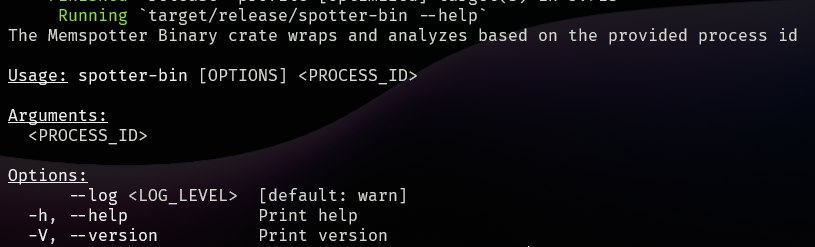
\includegraphics[width=0.5\linewidth]{cli-help.png}
        \caption{Running the binary with "--help" command}
        \label{fig:cli-help}
    \end{figure}

\subsection{the main interface}

After the program successfully launches, the user is shown the main interface, which consists of three parts: the code section, the picker section, and the header section.
The header is responsible for showing the id of the process being analyzed as well as the basic usage of the application.
The code and picker section alternate between active and passive states, which are changed by using the left and right arrow buttons.
The section that is currently active will take the vertical arrow button input for scrolling and active section selection. 
The code section is a window into the assembly instructions of the currently open linked library, it allows for scrolling and highlights the actively selected item and highlights all of the generated insights side by side with the respective instructions.
The picker section is responsible for facilitating user navigation; there the user can change which library to view in the code section.
Additionally, by detecting for the usage of the tab key when active the picker section transforms into a list of available function symbols in the active library, which allows the end user for easy jump across the library's code.
The highlight of this interface implementation is the management of the code section state as it needs to hold the entirety of assembly instructions for the library, which can be in tens of thousands of annotated instructions.
As the use interface in terminal interfaces needs to be fully refreshed upon every interaction, reloading this large amounts of code initially caused the application to significantly lag.
To combat this the code section has a given buffer size and offset, and through the use of own scroll functions (\autoref{lst:tui-scroll}) the buffer is adjusted when needed keeping the unseen parts of code from hindering the user interface's performance.

\begin{lstlisting}[caption=\label{lst:tui-scroll}"Custom overlays over the basic scroll functions", language=Rust]
    fn select_next(&mut self) {
        if let Some(i) = self.state.selected() {
            let diff = self.ctx_size - i;
            if diff <= self.render_cutoff {
                let select_offset = i - self.state.offset();
                self.offset += select_offset;
                self.state.select(Some(select_offset));
                *self.state.offset_mut() = 0;
            } else {
                self.state.select_next();
            }
        } else {
            self.offset = 0;
            self.state.select(Some(0));
        }
    }

    fn select_previous(&mut self) {
        if let Some(i) = self.state.selected() {
            if i == 0 && self.offset != 0 {
                self.offset = self.offset.saturating_sub(self.render_cutoff);
                self.state.select(Some(self.render_cutoff));
                *self.state.offset_mut() = self.render_cutoff;
            } else {
                self.state.select_previous();
            }
        } else {
            self.offset = 0;
            self.state.select(Some(0));
        }
    }
\end{lstlisting}

\section{Enforcement of clean code principles}
\label{clean_code}

    \subsection{Forbidding of unsafe code}
    
    Although rust is by definition a memory safe language due to the enforcement of the borrow checker and it's rules \cite{klabnik_rust_2023}. However, these features can be bypassed by using \verb|unsafe| code blocks, which disable these protection features at the programmer's request.
    In the case of this project, in order to enforce strict memory protection and avoid undefined behavior, the \verb|unsafe_code| lint has been set to \verb|forbid| level which makes any usage of the unsafe blocks in the produced code emit a compile-time error which in no way can be overridden \cite{klabnik_rust_2023}

    \subsection{Denying the use of unwrap function calls}

    One of the core features of the rust programming language is its verbosity in handling error cases, if a function can fail it usually returns a \verb|Result| which contains either the desired value or the error and needs to be handled appropriately \cite{klabnik_recoverable_2023}. The same is applied for possible null values that have been handled with the \verb| Option| type that returns a \verb| None| variant to signify the lack of a result. 
    Those enforcements can be quickly bypassed by calling \verb|.unwrap()| on a \verb|Result| or an \verb|Option| value which will force the program to produce the desired value or fail and panic in the other case.
    To ensure better code quality and fewer panics in implementation, the \verb|unwrap_used| lint has been set at the \verb|deny| level. 
    This makes use of any \verb|unwrap| function calls result in a compilation error which forces the programmer to either handle the possible errors and None value accordingly or use the more verbose \verb|.expect() | call, which requires an explanation to be provided as to why the program should not panic when unwrapping this value (\cite{klabnik_recoverable_2023}). 
    Furthermore, setting the \verb| expect_used| lint at a warning level will notify the programmer upon compilation that this method is not the best practice.

    \subsection{Requirement of Code Documentation and Other Lints}

    By setting the \verb|missing_docs| lint at a deny level the compiler will enforce that any public facing struct, enum, trait, and method needs to provide any documentation in order for the program to compile. This ensures that the code not only needs to be correct, but also documented in order to be compiled and tested, which results in better documented and more maintainable code. 
    Furthermore, by setting more specific lints such as \verb|clippy::pedantic| or \verb|clippy::nursery| the programmer is warned about bad code practices such as duplication module name in function or struct names or using less readable patterns such as \verb|if a != b|.

\section{Custom error types}

Using \verb|thiserror| crate's \cite{tolnay_dtolnaythiserror_2024} modules, the reader\autoref{reader} and the analyzer \autoref{analyzer} expose custom error types that allow better handling and display of any errors that occur. 
A good example of this is trying to read the memory of a process running with privileged access as a regular user (see \autoref{lst:verbose_err}). Normally, the resulted panic message would contain only the IO error produced by the access denied system response, but with custom error type, the message is more verbose.

\begin{lstlisting}[caption=\label{lst:verbose_err}"Error when trying to read the pid 1 process"]
Running `target/release/spotter-bin --log=error 1`
thread 'main' panicked at bin/src/main.rs:33:53:
Analyzer should init: Builder(
    Reader(
        MemFile(
            Parser(
                Os { code: 13, kind: PermissionDenied, message: "Permission denied" }
                ))))
\end{lstlisting}

Furthermore, this allows libraries that may depend on functions that emit such verbose errors to better respond to their occurrences and react accordingly. 
A good example of this is in the implementation of the \verb|x86_64| map trait \autoref{reader:map} in which the error thrown on the failure to parse a file that is not in a compatible format is caught and only emitted as a warning message instead of causing the entire program to panic.

\begin{lstlisting}[caption=\label{lst:err_handling}"Customm error handling example", language=Rust]
let lib = match Library::try_from(p.clone()) {
                Ok(lib) => lib,
                Err(e) => {
                    tracing::warn!(
                        "failure to parse file {} skipping function extraction ({})",
                        p.display(),
                        e
                    );
                    continue;
                }
            };
\end{lstlisting}

Additionally, by using custom error types, the program test suite can be enhanced with purposefully panicking code which passes the test only on specific error types.

\section{Tracing}

By incorporating the \verb|tracing| \cite{tokio-rs_team_tokio-rstracing_2024} dependency into the reader \autoref{reader} and analyzer \autoref{analyzer} modules, the exposed methods can produce tracing information that can be used and consumed by other libraries.

\begin{lstlisting}[language=Rust, caption="Code fragment showcasing conditionally emiting a warning"]
if let Some(rep) = map.insert(addr, f.clone()) {
    tracing::warn!("clashing addresses replaced {:?} with {:?}", rep, f);
}
\end{lstlisting}

The binary module uses the \verb|tracing_subscriber| \cite{tokio-rs_team_tokiotracingtracing-subscriber_2024} crate to consume the data provided by it's function as well as it's dependencies, and with the CLI setup to allow for trace level filtering the program can emit desired information to the end user.

\begin{lstlisting}[breaklines=true, caption="Fraction of the warnings emitted by the program with the log setting at warning level"]
$ cargo run --release -- --log=warn 5293
...
2025-01-05T15:27:26.763134Z  WARN func_map{lib="ld-linux-x86-64.so.2"}: memspotter_analyzer::diff_analyzer: clashing addresses replaced sbrk 0x22d10[139] with __sbrk 0x22d10[139]
2025-01-05T15:27:26.763153Z  WARN func_map{lib="ld-linux-x86-64.so.2"}: memspotter_analyzer::diff_analyzer: clashing addresses replaced __GI_mprotect 0x24800[36] with mprotect 0x24800[36]
2025-01-05T15:27:26.763172Z  WARN func_map{lib="ld-linux-x86-64.so.2"}: memspotter_analyzer::diff_analyzer: clashing addresses replaced access 0x241c0[55] with __access 0x241c0[55]
2025-01-05T15:27:26.763191Z  WARN func_map{lib="ld-linux-x86-64.so.2"}: memspotter_analyzer::diff_analyzer: clashing addresses replaced __closedir 0x22e80[44] with closedir 0x22e80[44]
2025-01-05T15:27:26.763211Z  WARN func_map{lib="ld-linux-x86-64.so.2"}: memspotter_analyzer::diff_analyzer: clashing addresses replaced __GI___fstatat 0x24240[76] with __GI___fstatat64 0x24240[76]
\end{lstlisting}
    \chapter{Results}
\label{cha:results}

\section{Example Analysis - the `top` process}

\subsection{Brief UI overview}

\subsection{Analyzing the main library}

\subsection{Main function and its calls}

\subsection{Brief look at dependencies}

\subsection{Looking at compiler/linker optimizations and it's possible effects}
    \chapter{Conclusions}
\label{cha:conlusions}

\section{Highlights}

\begin{enumerate}
    \item{Memory Map} 
    
    The abstraction created for the process memory map was done very diligently and the techniques used, such as smart pointers, allowed for a very quick and memory-efficient implementation.
    Additionally, providing data structures which joined library and raw memory data enhanced the reader's overall ease of use and allowed for smooth memory address translation that was needed in analysis. 

    \item{Library and Memory address translation}

    The mechanism for address translation, between memory space and process addressing, was also well implemented.
    Furthermore, by allowing the function struct (\autoref{lst:so-function}) to hold the memory offset as well as function's virtual address and size, the analysis capabilities of the program could be easily extended to length verification or even creating function checksums for easier comparison.

    \item{User interface}

    The application being a terminal interface allows usage in any environment and supports most common terminals. 
    Furthermore, usage of colors and highlighting allows for a clean and easy-to-read interface.
    Additionally, by implementing app navigation without mouse support and for keyboard keys the application can be easily used even through ssh connections.

    \item {Function call matching}
    By creating a global hash map of all function signatures, the program can quickly and effectively match memory addresses to function names, significantly speeding up the analysis process.
    Furthermore, by making the hash map global if the program is extended with procedure linkage table section analysis, this would allow for automatic matching of cross-library function calls without sacrificing the applications speed or requiring significant codebase upgrades.

    \item{Core testing}
    To ensure the correctness of the software, the core codebase is extensively unit tested with the reader crate having 18 unit and integration test to verify the workings and a 57\% (over 72\% for the reader module!) test code coverage. 
    This is vital for ensuring that all of the core functionality works as expected and allows for easier future development as any new extensions or enhancements can be tested against the core functionality.

    \begin{lstlisting}[caption="reader and analyzer joined coverage results"]
    2025-01-11T21:25:28.742084Z  INFO cargo_tarpaulin::report: Coverage Results:
|| Tested/Total Lines:
|| analyzer/src/diff_analyzer.rs: 0/58 +0.00%
|| analyzer/src/difference.rs: 0/26 +0.00%
|| analyzer/src/insight.rs: 0/11 +0.00%
|| analyzer/src/instruction.rs: 0/10 +0.00%
|| reader/src/permissions.rs: 20/20 +0.00%
|| reader/src/segments/break.rs: 11/18 +0.00%
|| reader/src/segments/heap.rs: 11/18 +0.00%
|| reader/src/segments/linked.rs: 13/18 +0.00%
|| reader/src/segments/mapped_object.rs: 19/36 +0.00%
|| reader/src/segments/stack.rs: 10/17 +0.00%
|| reader/src/segments/vdso.rs: 3/10 +0.00%
|| reader/src/segments/vvar.rs: 3/10 +0.00%
|| reader/src/x86_64/header.rs: 32/36 +0.00%
|| reader/src/x86_64/map.rs: 51/53 +0.00%
|| reader/src/x86_64/segment.rs: 20/31 +0.00%
|| reader/src/x86_64/shared_object.rs: 60/82 +0.00%
|| reader/src/x86_64/so_function.rs: 19/28 +0.00%
|| reader/tests/common/mod.rs: 10/10 +0.00%
||
57.32% coverage, 282/492 lines covered, +0.00% change in coverage
    \end{lstlisting}
    
\end{enumerate}

\section{Shortcomings}

\begin{enumerate}

    \item {Lack of wider section analysis}
    
    Even though the program does really well in analyzing the executable section of the provided process, the analysis of the procedure linkage table or readable and writable data sections could provide more insights, such as user-set variables or program's static string.
    However, this would require innate knowledge or parsing of data structures on a library basis, which is immensely hard and tedious to implement even for a single architecture set.
    
    \item{Basic address collision resolution}

    The app provides only the basic function address collision resolution with the last function signature encountered to remain.
    This process could have been implemented better, e.g. by collecting all of the colliding function names and displaying them, as the current implementation leaves this data only as warnings in the program logs. 

    \item{No Demangling support}

    The reader module parses the data from the symbol string table as-is, which means that C libraries developed with long namespaces or in different languages will provide less readable function names which could harm the user experience.
    However, the basic function names can still always be readable, which does not hurt much of the program's functionality. 
    
\end{enumerate}

\section{Possible future enhancements}

\begin{enumerate}
    \item{Additional architecture support}

    Implementing the new architectures could be as simple as providing a new map trait implementation for 32-bit Linux systems, which would significantly widen the program's usage cases.
    Furthermore, even implementing very varying architectures can be implemented without rewriting singinficant amount of the codebase due to the project's modularity, the analyzer's basic string output type, and the terminal interface style being very cross-platform compatible.
    
    \item {Basic C/C++ demangling}

    Implementing basic demangling for linked libraries based on C or C++ could be as easy as plugging a demangling library into the function creation process.
    Or, if such library is unavailable for the Rust language, then implementing the functionality through the usage of FFI calls.
    This would wildly enhance the program's analysis capabilities as multiple programming languages also rely on C based libraries, especially on Linux systems.

    \item {Cross-library and cross-segment function call tracing}

    By implementing analysis for the procedure linkage table of linked libraries, the program could very easily recognize the function call made to other libraries and make the process of process analysis significantly more streamlined.
    Furthermore, this capability could be extended with interface functionality, e.g. jumping to the called function on a button press which would make tracing the process execution path trivial.
    
\end{enumerate}

    
	% itd.
	\appendix
	% \include{dodatekA}
	% \include{dodatekB}
	% itd.
	
	\printbibliography

\end{document}
